\documentclass[preprint,12pt,aps,pra,showkeys,amsmath,amssymb,superscriptaddress,floatfix]{revtex4-2}
\usepackage[T1]{fontenc}
\usepackage[utf8]{inputenc}
\usepackage{amsmath,amssymb,amsthm,mathtools,mathrsfs}
\usepackage{microtype,booktabs,enumitem}
\usepackage{xcolor,tikz,etoolbox}
\usepackage[skins,breakable]{tcolorbox}
\usepackage{needspace}
% Keep diagram geometry independent of REVTeX preprint body spacing.
\AtBeginEnvironment{tikzpicture}{\linespread{1}\selectfont}
\usetikzlibrary{arrows.meta,positioning,calc,fit,decorations.pathreplacing}
\usepackage{graphicx}
\usepackage{hyperref}

\definecolor{MMBlue}{RGB}{0,82,155}
\definecolor{MMOrange}{RGB}{200,80,0}
\tikzset{
 mmnode/.style={draw=MMBlue,rounded corners=2pt,fill=MMBlue!4,align=left,execute at begin node={\raggedright},text width=5cm,font=\fontsize{10}{12}\selectfont,inner sep=6pt},
 mmimport/.style={mmnode,draw=black!65,fill=black!4},
 mmcandidate/.style={mmnode,draw=MMOrange,dashed,fill=MMOrange!5},
 mmrejected/.style={mmnode,draw=black,densely dotted,fill=black!8},
 mmproof/.style={->,thick,MMBlue},
 mmflow/.style={->,semithick,black!70},
 mmrepair/.style={->,dashed,thick,MMOrange},
 mmcandidatearrow/.style={->,dashed,semithick,MMOrange},
 mmnote/.style={font=\scriptsize,fill=white,inner sep=2pt,align=center}}

\usepackage[section]{placeins}
\setlength{\emergencystretch}{3em}
\setlist{itemsep=3pt,topsep=4pt}
\newtheorem{theorem}{Theorem}[section]
\newtheorem{proposition}[theorem]{Proposition}
\newtheorem{lemma}[theorem]{Lemma}
\newtheorem{corollary}[theorem]{Corollary}
\theoremstyle{definition}
\newtheorem{definition}[theorem]{Definition}
\newtheorem{example}[theorem]{Example}
\theoremstyle{remark}
\newtheorem{remark}[theorem]{Remark}
% Avoid isolated statement headings and single-line paragraph fragments.
\BeforeBeginEnvironment{theorem}{\Needspace{6\baselineskip}}
\BeforeBeginEnvironment{definition}{\Needspace{5\baselineskip}}
\BeforeBeginEnvironment{proposition}{\Needspace{5\baselineskip}}
\BeforeBeginEnvironment{lemma}{\Needspace{5\baselineskip}}
\BeforeBeginEnvironment{corollary}{\Needspace{5\baselineskip}}
\clubpenalty=5000
\widowpenalty=5000
\newcommand{\R}{\mathbb R}\newcommand{\Z}{\mathbb Z}\newcommand{\N}{\mathbb N}
\newcommand{\Pa}{\operatorname{Pa}}\newcommand{\Desc}{\operatorname{Desc}}
\newcommand{\cl}{\operatorname{cl}}\newcommand{\cost}{\operatorname{cost}}
\newcommand{\status}{\operatorname{status}}
% Faculty cards: a visual rail groups the five faculties within one agent.
% The rail has no arrowhead and does not represent a proof dependency.
\newcommand{\mmfacultybadge}[1]{%
 \node[circle,draw=MMBlue,line width=1pt,fill=white,
 minimum size=7mm,inner sep=0pt,font=\sffamily\small\bfseries,text=MMBlue]
 at ([xshift=15pt,yshift=-15pt]frame.north west) {#1};}
\newcommand{\mmfacultyrail}{%
 \draw[MMBlue!80,line width=1pt]
 ([xshift=15pt,yshift=2pt]frame.north west)--
 ([xshift=15pt,yshift=-2pt]frame.south west);}
\newtcolorbox{mmfacultybox}[2]{enhanced,breakable,
 colback=MMBlue!4,colframe=MMBlue!4,boxrule=0pt,arc=3pt,
 left=39pt,right=9pt,top=4pt,bottom=4pt,
 before skip=2pt,after skip=2pt,
 fontupper=\small\linespread{1.1}\selectfont,
 overlay unbroken={\mmfacultyrail\mmfacultybadge{#1}},
 overlay first={\mmfacultyrail\mmfacultybadge{#1}},
 overlay middle={\mmfacultyrail},overlay last={\mmfacultyrail}}
\newcommand{\mmfaculty}[3]{%
 \begin{mmfacultybox}{#1}{#2}
 {\sffamily\bfseries\color{MMBlue}#2}\par\smallskip #3
 \end{mmfacultybox}}
\newcommand{\agent}[9]{%
 \Needspace{8\baselineskip}
 \subsubsection{#1}
 \noindent\textbf{Object.} #2\par
 \noindent\textbf{Role.} #3\par\smallskip
 \mmfaculty{E}{Ego}{#4}
 \mmfaculty{M}{Memory}{#5}
 \mmfaculty{I}{Intellect}{#6}
 \mmfaculty{S}{Sense}{#7}
 \mmfaculty{A}{Action}{#8}
 \smallskip\noindent #9\par}

\usepackage{longtable,array,calc}
\providecommand{\tightlist}{\setlength{\itemsep}{2pt}\setlength{\parskip}{0pt}}
\makeatletter
\def\frontmatter@abstract@produce{\par\addvspace{\frontmatter@preabstractspace}%
\begingroup\prep@absbox\unvbox\absbox\post@absbox\endgroup
\addvspace{\frontmatter@postabstractspace}}
\makeatother
\newcommand{\field}[2]{\par\smallskip\noindent\textbf{#1.} #2\par}
\setlength{\emergencystretch}{5em}
\AtBeginEnvironment{verbatim}{\small\linespread{1.0}\selectfont}


\hypersetup{colorlinks=true,linkcolor=MMBlue,urlcolor=MMBlue,pdfauthor={Dibakar Sigdel}}

\begin{document}

\title{Fundamental Theorem of Galois Theory\\[4pt]\large An End-to-End Meta-Math Walkthrough}

\author{Dibakar Sigdel}

\affiliation{Mindverse Computing LLC, Lynnwood, WA 98087, USA}

\date{October 2026}

\begin{abstract}

A complete authored walkthrough of fundamental theorem of galois theory,
with explicit mathematical contracts, local verification gates, and
reusable exports. The report presents the target theorem, declared
imports, a dependency graph, five-faculty node contracts, a continuous
proof, a worked example, and a hypothesis-repair audit. It is an
authored mathematical exposition, not a deployed-agent transcript or a
formal proof-assistant certificate.

\end{abstract}\maketitle\linespread{1.12}\selectfont

\noindent\textbf{MA-04 / Modern Algebra / Report v1}

\section{Target and import contract}

\begin{theorem}

For a finite Galois extension \(L/K\) with group \(G\), prove an
inclusion-reversing bijection between intermediate fields \(E\) and
subgroups \(H\le G\), via \(E\mapsto\operatorname{Gal}(L/E)\) and
\(H\mapsto L^H\). Prove \([L:L^H]=|H|\) and normal subgroups correspond
to intermediate extensions Galois over K, with quotient group \(G/H\).

\end{theorem}

\subsection{Foundations and permitted imports}

L/K is a finite normal separable extension,
\(G=\operatorname{Aut} _K(L)\). Import: (i) finite Galois extensions
have automorphism count equal to degree; (ii) Artin's fixed-field
theorem, for a finite automorphism subgroup H, \([L:L^H]=|H|\) and
\(L/L^H\) is Galois; (iii) the tower law; (iv) embeddings of an
intermediate field into an algebraic closure extend to L, and
K-normality sendsL to itself. These are substantive field-theory
imports, not the correspondence being proved.

The last step also imports the first isomorphism theorem (MA-02).

\clearpage\section{Node interaction workflow}

\begin{center}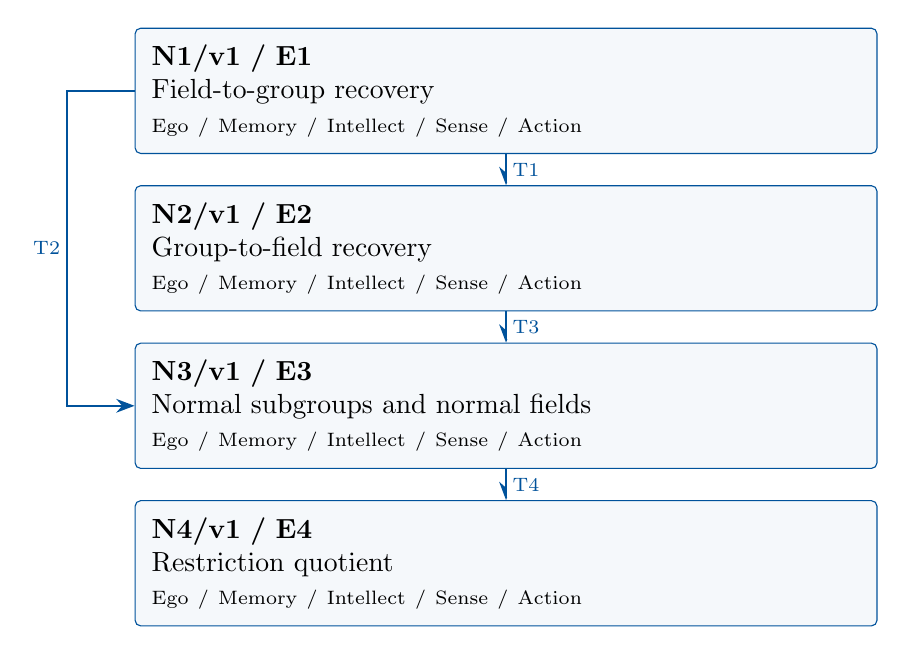
\begin{tikzpicture}[>=Stealth,x=1cm,y=1cm]

\node[mmnode,text width=9cm,minimum height=1.25cm] (N1) at (0,0.0) {\textbf{N1/v1 / E1}\\Field-to-group recovery\\{\scriptsize Ego / Memory / Intellect / Sense / Action}};

\node[mmnode,text width=9cm,minimum height=1.25cm] (N2) at (0,-2.0) {\textbf{N2/v1 / E2}\\Group-to-field recovery\\{\scriptsize Ego / Memory / Intellect / Sense / Action}};

\node[mmnode,text width=9cm,minimum height=1.25cm] (N3) at (0,-4.0) {\textbf{N3/v1 / E3}\\Normal subgroups and normal fields\\{\scriptsize Ego / Memory / Intellect / Sense / Action}};

\node[mmnode,text width=9cm,minimum height=1.25cm] (N4) at (0,-6.0) {\textbf{N4/v1 / E4}\\Restriction quotient\\{\scriptsize Ego / Memory / Intellect / Sense / Action}};

\draw[mmproof] (N1.south) -- node[mmnote,right] {T1} (N2.north);

\draw[mmproof] (N1.west) -- (-5.58,0) -- node[mmnote,left] {T2} (-5.58,-4) -- (N3.west);

\draw[mmproof] (N2.south) -- node[mmnote,right] {T3} (N3.north);

\draw[mmproof] (N3.south) -- node[mmnote,right] {T4} (N4.north);

\end{tikzpicture}\end{center}

Each box is one mathematical agent containing all five faculties. Blue
arrows carry the versioned exports listed below. The layout gives a
reading order; only drawn arrows assert dependencies. Diagnostic repair
is separate from the proof DAG.

\clearpage\subsection{Versioned evidence-transfer ledger}

\begingroup\small\linespread{1.05}\selectfont

\Needspace{5\baselineskip}\field{T1: N1/E1/v1 to N2}{The field recovered from its fixing subgroup is exactlyE.}

\field{Receiving activity}{N2: Group-to-field recovery}

\field{Compatibility}{Use the same mathematical objects and hypotheses as the source export.
Receiving contract: SubgroupH \(\le G\); \(E_H=L^H\); prior exports
E1/v1}

\Needspace{5\baselineskip}\field{T2: N1/E1/v1 to N3}{The field recovered from its fixing subgroup is exactlyE.}

\field{Receiving activity}{N3: Normal subgroups and normal fields}

\field{Compatibility}{Use the same mathematical objects and hypotheses as the source export.
Receiving contract: Correspondence and extension of embeddings; prior
exports E1/v1, E2/v1}

\Needspace{5\baselineskip}\field{T3: N2/E2/v1 to N3}{Both inverse identities and the degree \(formula[L:L^H]=|H|\).}

\field{Receiving activity}{N3: Normal subgroups and normal fields}

\field{Compatibility}{Use the same mathematical objects and hypotheses as the source export.
Receiving contract: Correspondence and extension of embeddings; prior
exports E1/v1, E2/v1}

\Needspace{5\baselineskip}\field{T4: N3/E3/v1 to N4}{H normal in G iff its fixed field is Galois over K.}

\field{Receiving activity}{N4: Restriction quotient}

\field{Compatibility}{Use the same mathematical objects and hypotheses as the source export.
Receiving contract: NormalH and \(E=L^H\); prior exports E3/v1}

\endgroup

\clearpage\section{Agent roles and five-faculty activities}\begingroup\small\linespread{1.05}\selectfont\setlist{itemsep=1pt,topsep=2pt}

\subsection{N1/v1: Field-to-group recovery}

\field{Object and role}{Compare degrees after forming its fixing subgroup.}

\field{Inputs}{Intermediate \(K\subset E\subset L\); foundational imports stated in §1}

\mmfaculty{E}{Ego}{Own E1/v1: The field recovered from its fixing subgroup is exactlyE.}

\mmfaculty{M}{Memory}{Retain Intermediate \(K\subset E\subset L\); foundational imports stated
in §1; keep their assumptions and versions attached.}

\mmfaculty{I}{Intellect}{Compare degrees after forming its fixing subgroup.}

\mmfaculty{S}{Sense}{Inclusion alone is not enough; degree equality closes recovery.}

\mmfaculty{A}{Action}{Carry out the numbered deductions and publish E1/v1 together with its
hypotheses and proof location.}

\smallskip\noindent\textbf{Numbered mathematical activities}

\begin{enumerate}[label=N1.\arabic*,leftmargin=3.4em]

\item L/E remains normal and separable: L is a splitting field over K of
separable polynomials and hence also a splitting field of those
polynomials over E.

\item Set \(H_E=\operatorname{Aut} _E(L)\); the automorphism-count import
\(gives|H_E|=[L:E]\).

\item Certainly \(E\subset L^{H_E}\).

\item Artin \(gives[L:L^{H_E}]=|H_E|=[L:E]\).

\item The tower law then \(forces[L^{H_E}:E]=1\), so \(L^{H_E}=E\).

\end{enumerate}

\field{Export E1/v1}{The field recovered from its fixing subgroup is exactlyE.}

\field{Acceptance gate}{Inclusion alone is not enough; degree equality closes recovery. Publish
only after checking every displayed deduction.}

\field{Targeted repair}{If the check fails, revise N1: Inclusion alone is not enough; degree
equality closes recovery. Recheck dependent nodes N2, N3, N4.}

\clearpage

\subsection{N2/v1: Group-to-field recovery}

\field{Object and role}{Compare the group sizes supplied by Artin.}

\field{Inputs}{SubgroupH \(\le G\); \(E_H=L^H\); prior exports E1/v1}

\mmfaculty{E}{Ego}{Own E2/v1: Both inverse identities and the degree
\(formula[L:L^H]=|H|\).}

\mmfaculty{M}{Memory}{Retain SubgroupH \(\le G\); \(E_H=L^H\); prior exports E1/v1; keep their
assumptions and versions attached.}

\mmfaculty{I}{Intellect}{Compare the group sizes supplied by Artin.}

\mmfaculty{S}{Sense}{Fixing all of E is stronger than preservingE as a set.}

\mmfaculty{A}{Action}{Carry out the numbered deductions and publish E2/v1 together with its
hypotheses and proof location.}

\smallskip\noindent\textbf{Numbered mathematical activities}

\begin{enumerate}[label=N2.\arabic*,leftmargin=3.4em]

\item H fixes \(E_H\) pointwise, so \(H\subset \operatorname{Aut} _{E_H}(L)\).

\item Artin says \(L/E_H\) is Galois and its degree is\textbar H\textbar.

\item Thus its full automorphism group has\textbar H\textbar{} elements and
equals H.

\item The two constructions are therefore mutual inverses.

\item If \(E_{1}\subset E_{2}\) then every automorphism fixing \(E_{2}\) fixes
\(E_{1}\), so \(H_{E_{2}}\subset H_{E_{1}}\); if \(H_{1}\subset H_{2}\)
then \(L^{H_{2}}\subset L^{H_{1}}\).

\item This proves the inclusion-reversing bijection.

\end{enumerate}

\field{Export E2/v1}{Both inverse identities and the degree \(formula[L:L^H]=|H|\).}

\field{Acceptance gate}{Fixing all of E is stronger than preservingE as a set. Publish only
after checking every displayed deduction.}

\field{Targeted repair}{If the check fails, revise N2: Fixing all of E is stronger than
preservingE as a set. Recheck dependent nodes N3, N4.}

\clearpage

\subsection{N3/v1: Normal subgroups and normal fields}

\field{Object and role}{Translate conjugation to stability of the fixed field.}

\field{Inputs}{Correspondence and extension of embeddings; prior exports E1/v1, E2/v1}

\mmfaculty{E}{Ego}{Own E3/v1: H normal in G iff its fixed field is Galois over K.}

\mmfaculty{M}{Memory}{Retain Correspondence and extension of embeddings; prior exports E1/v1,
E2/v1; keep their assumptions and versions attached.}

\mmfaculty{I}{Intellect}{Translate conjugation to stability of the fixed field.}

\mmfaculty{S}{Sense}{All embeddings, not just a few automorphisms, must be controlled.}

\mmfaculty{A}{Action}{Carry out the numbered deductions and publish E3/v1 together with its
hypotheses and proof location.}

\smallskip\noindent\textbf{Numbered mathematical activities}

\begin{enumerate}[label=N3.\arabic*,leftmargin=3.4em]

\item For \(\sigma \in G\), the fixing subgroup of \(\sigma (E)\) is
\(\sigma H_E\sigma ^{-1}\), so the correspondence makes \(H_E\) normal
exactly when \(\sigma (E)=E\) for every \(\sigma\).

\item If E/K is normal, each such \(\sigma\) preserves E.

\item Conversely every K-embedding of E extends to aK-embedding of L and thus
to an element of G; stability then makes all conjugates of E equal E,
proving normality.

\item Separability descends from L/K, so this is precisely the Galois
condition on E/K.

\end{enumerate}

\field{Export E3/v1}{H normal in G iff its fixed field is Galois over K.}

\field{Acceptance gate}{All embeddings, not just a few automorphisms, must be controlled.
Publish only after checking every displayed deduction.}

\field{Targeted repair}{If the check fails, revise N3: All embeddings, not just a few
automorphisms, must be controlled. Recheck dependent nodes N4.}

\clearpage

\subsection{N4/v1: Restriction quotient}

\field{Object and role}{Check surjectivity using embedding extension.}

\field{Inputs}{NormalH and \(E=L^H\); prior exports E3/v1}

\mmfaculty{E}{Ego}{Own E4/v1: The normal-field quotient identification
\(G/H\cong \operatorname{Gal} (E/K)\).}

\mmfaculty{M}{Memory}{Retain NormalH and \(E=L^H\); prior exports E3/v1; keep their
assumptions and versions attached.}

\mmfaculty{I}{Intellect}{Check surjectivity using embedding extension.}

\mmfaculty{S}{Sense}{Without normality restriction need not land in
\(\operatorname{Aut} _K(E)\).}

\mmfaculty{A}{Action}{Carry out the numbered deductions and publish E4/v1 together with its
hypotheses and proof location.}

\smallskip\noindent\textbf{Numbered mathematical activities}

\begin{enumerate}[label=N4.\arabic*,leftmargin=3.4em]

\item Restriction \(\operatorname{res} :G\to \operatorname{Aut} _K(E)\) is
defined because E is stable.

\item Its kernel consists exactly of automorphisms fixing E, namelyH.

\item AnyK-automorphism of E extends to L; normality of L/K makes the
extension an element of G, so res is onto.

\item By MA-02,
\(G/H\cong \operatorname{Aut} _K(E)=\operatorname{Gal} (E/K)\).

\item This closes the entire theorem.

\end{enumerate}

\field{Export E4/v1}{The normal-field quotient identification
\(G/H\cong \operatorname{Gal} (E/K)\).}

\field{Acceptance gate}{Without normality restriction need not land in
\(\operatorname{Aut} _K(E)\). Publish only after checking every
displayed deduction.}

\field{Targeted repair}{If the check fails, revise N4: Without normality restriction need not
land in \(\operatorname{Aut} _K(E)\). Withhold this terminal result
until its gate passes.}

\endgroup\clearpage\section{Continuous mathematical proof}\label{sec:proof}

Read these steps in order as one proof; the diagram is optional.
Numbered activities identify the specific constructions and deductions
owned by each node.

\subsection{§4.N1 --- Field-to-group
recovery}\label{n1-field-to-group-recovery}

\begin{enumerate}
\def\labelenumi{\arabic{enumi}.}
\item
  L/E remains normal and separable: L is a splitting field over K of
  separable polynomials and hence also a splitting field of those
  polynomials over E.
\item
  Set \(H_E=\operatorname{Aut} _E(L)\); the automorphism-count import
  \(gives|H_E|=[L:E]\).
\item
  Certainly \(E\subset L^{H_E}\).
\item
  Artin \(gives[L:L^{H_E}]=|H_E|=[L:E]\).
\item
  The tower law then \(forces[L^{H_E}:E]=1\), so \(L^{H_E}=E\).
\end{enumerate}

\subsection{§4.N2 --- Group-to-field
recovery}\label{n2-group-to-field-recovery}

\begin{enumerate}
\def\labelenumi{\arabic{enumi}.}
\item
  H fixes \(E_H\) pointwise, so
  \(H\subset \operatorname{Aut} _{E_H}(L)\).
\item
  Artin says \(L/E_H\) is Galois and its degree is\textbar H\textbar.
\item
  Thus its full automorphism group has\textbar H\textbar{} elements and
  equals H.
\item
  The two constructions are therefore mutual inverses.
\item
  If \(E_{1}\subset E_{2}\) then every automorphism fixing \(E_{2}\)
  fixes \(E_{1}\), so \(H_{E_{2}}\subset H_{E_{1}}\); if
  \(H_{1}\subset H_{2}\) then \(L^{H_{2}}\subset L^{H_{1}}\).
\item
  This proves the inclusion-reversing bijection.
\end{enumerate}

\subsection{§4.N3 --- Normal subgroups and normal
fields}\label{n3-normal-subgroups-and-normal-fields}

\begin{enumerate}
\def\labelenumi{\arabic{enumi}.}
\item
  For \(\sigma \in G\), the fixing subgroup of \(\sigma (E)\) is
  \(\sigma H_E\sigma ^{-1}\), so the correspondence makes \(H_E\) normal
  exactly when \(\sigma (E)=E\) for every \(\sigma\).
\item
  If E/K is normal, each such \(\sigma\) preserves E.
\item
  Conversely every K-embedding of E extends to aK-embedding of L and
  thus to an element of G; stability then makes all conjugates of E
  equal E, proving normality.
\item
  Separability descends from L/K, so this is precisely the Galois
  condition on E/K.
\end{enumerate}

\subsection{§4.N4 --- Restriction
quotient}\label{n4-restriction-quotient}

\begin{enumerate}
\def\labelenumi{\arabic{enumi}.}
\item
  Restriction \(\operatorname{res} :G\to \operatorname{Aut} _K(E)\) is
  defined because E is stable.
\item
  Its kernel consists exactly of automorphisms fixing E, namelyH.
\item
  AnyK-automorphism of E extends to L; normality of L/K makes the
  extension an element of G, so res is onto.
\item
  By MA-02,
  \(G/H\cong \operatorname{Aut} _K(E)=\operatorname{Gal} (E/K)\).
\item
  This closes the entire theorem.
\end{enumerate}

\hfill$\square$

\section{Worked orchestration}

Let \(L=Q(\sqrt{2},\sqrt{3)}\), \(K=Q\). The four sign changes form
\(C_{2}\times C_{2}\). The subgroup fixing \(\sqrt{2}\) consists of the
identity and the change \(\sqrt{3\mapsto }-\sqrt{3}\); its fixed field
is \(Q(\sqrt{2)}\), \(and[L:Q(\sqrt{2)]}=2=|H|\). All subgroups are
normal and the restriction quotient has order 2.

\subsection{Boundary and hypothesis audit}

\(Q(\sqrt[3]{}2)/Q\) is not normal: its nonreal conjugate roots are
absent and itsQ-automorphism group is trivial. Its fixed field under
that trivial group is the whole extension, notQ. Sense blocks using this
extension in the finite Galois correspondence.

\section{Illustrative failure and repair}

The following is an authored diagnostic scenario. Changed assumptions
define a new contract; they do not retroactively prove the original
statement.

\subsection{Failure and correction}
This is an authored teaching trace, not a recorded agent run.

\begin{enumerate}
\def\labelenumi{\arabic{enumi}.}
\tightlist
\item
  \textbf{Ego \(\to\) Memory:} register the §1 theorem, imports, and
  requested exports before beginning the proof.
\item
  \textbf{Intellect \(\to\) Action:} choose the bridges in §3 and carry
  out the numbered activities in §4; transmit only established E-exports
  along the §2 DAG.
\item
  \textbf{Sense \(\to\) responsible node:} test the specific
  boundary/failure in §5 and the node's individual audit. A failing
  candidate is withheld; downstream nodes may not use it.
\item
  \textbf{Memory + Intellect:} identify whether the error is an omitted
  condition, an invalid inference, or an attempted extension beyond the
  theorem. Restore the exact contract or explicitly state a different
  one.
\item
  \textbf{Action:} redo the affected mathematical activity using the
  repaired condition or inference. Recheck consuming nodes, rather than
  feeding their conclusions back as premises.
\item
  \textbf{Ego:} publish only the supported export with its assumptions
  and proof location. A hypothetical revised export is v2; the written
  proof here is the v1 exposition, not a claim that this repair was
  executed.
\end{enumerate}

\subsection{Hypothesis boundary}
\(Q(\sqrt[3]{}2)/Q\) is not normal: its nonreal conjugate roots are
absent and itsQ-automorphism group is trivial. Its fixed field under
that trivial group is the whole extension, notQ. Sense blocks using this
extension in the finite Galois correspondence.

\subsection{Version and recheck}
Treat any changed assumption as a new contract. Recheck the revised
export and all of its descendants. A backward diagnostic never
establishes an earlier theorem. This is an authored teaching trace, not
an execution log.

\par\medskip\begingroup\small\linespread{1.0}\selectfont\noindent\textbf{Provenance.} This authored proof is complete relative to its declared imports. Reuse
each export with its assumptions, proof, and version. The original
Markdown remains available for comparison.
\par\endgroup

\par\smallskip\begingroup\small\linespread{1.0}\selectfont\noindent\textbf{Further reading.} \begin{itemize}
\tightlist
\item
  \href{https://ocw.mit.edu/courses/res-18-012-algebra-ii-student-notes-spring-2022/pages/student-notes/}{MIT
  Algebra II notes: field extensions and Galois theory}.
\end{itemize}\par\endgroup

\end{document}
